\documentclass{ctexart}
\usepackage{graphicx}

\graphicspath{{figures/}}


\begin{document}
    % 浮动体
    % 实现灵活分页(避免无法分割的内容产生的页面留白)
    % 给图表添加艾标题
    % 交叉引用

    % figure环境(table环境与之类似)
    % \begin{figure}[<允许位置>]
    %     <任意内容>
    % \end{figure}

    % <允许位置>参数(默认tbp)
    % h,此处(here) 代码所在的上下文位置
    % t,页顶(top) 代码所在页面或之后页面的顶部
    % b,页底(bottom),代码所在页面或之后页面的底部
    % p,独立一页(page) 浮动页面

    % 标题控制(caption、bicaption等宏包)
    % 并排与字图表(subcaption、subfig、floatrow等宏包)
    % 绕排(picinpar、wrapfig等宏包)
    
    \LaTeX{}中的\TeX 系统的吉祥物---小狮子见图\ref{fig-lion}
    \begin{figure}[htbp]
        \centering
        
\includegraphics[scale=0.3]{lion}
        \caption{\TeX 系统吉祥物---小狮子}\label{fig-lion}
    \end{figure}

    遥望太白(?),看积雪皑皑,别有一番风景(图\ref{fig-mountain})。
    \begin{figure}[htbp]  % 允许各个位置
        \centering
        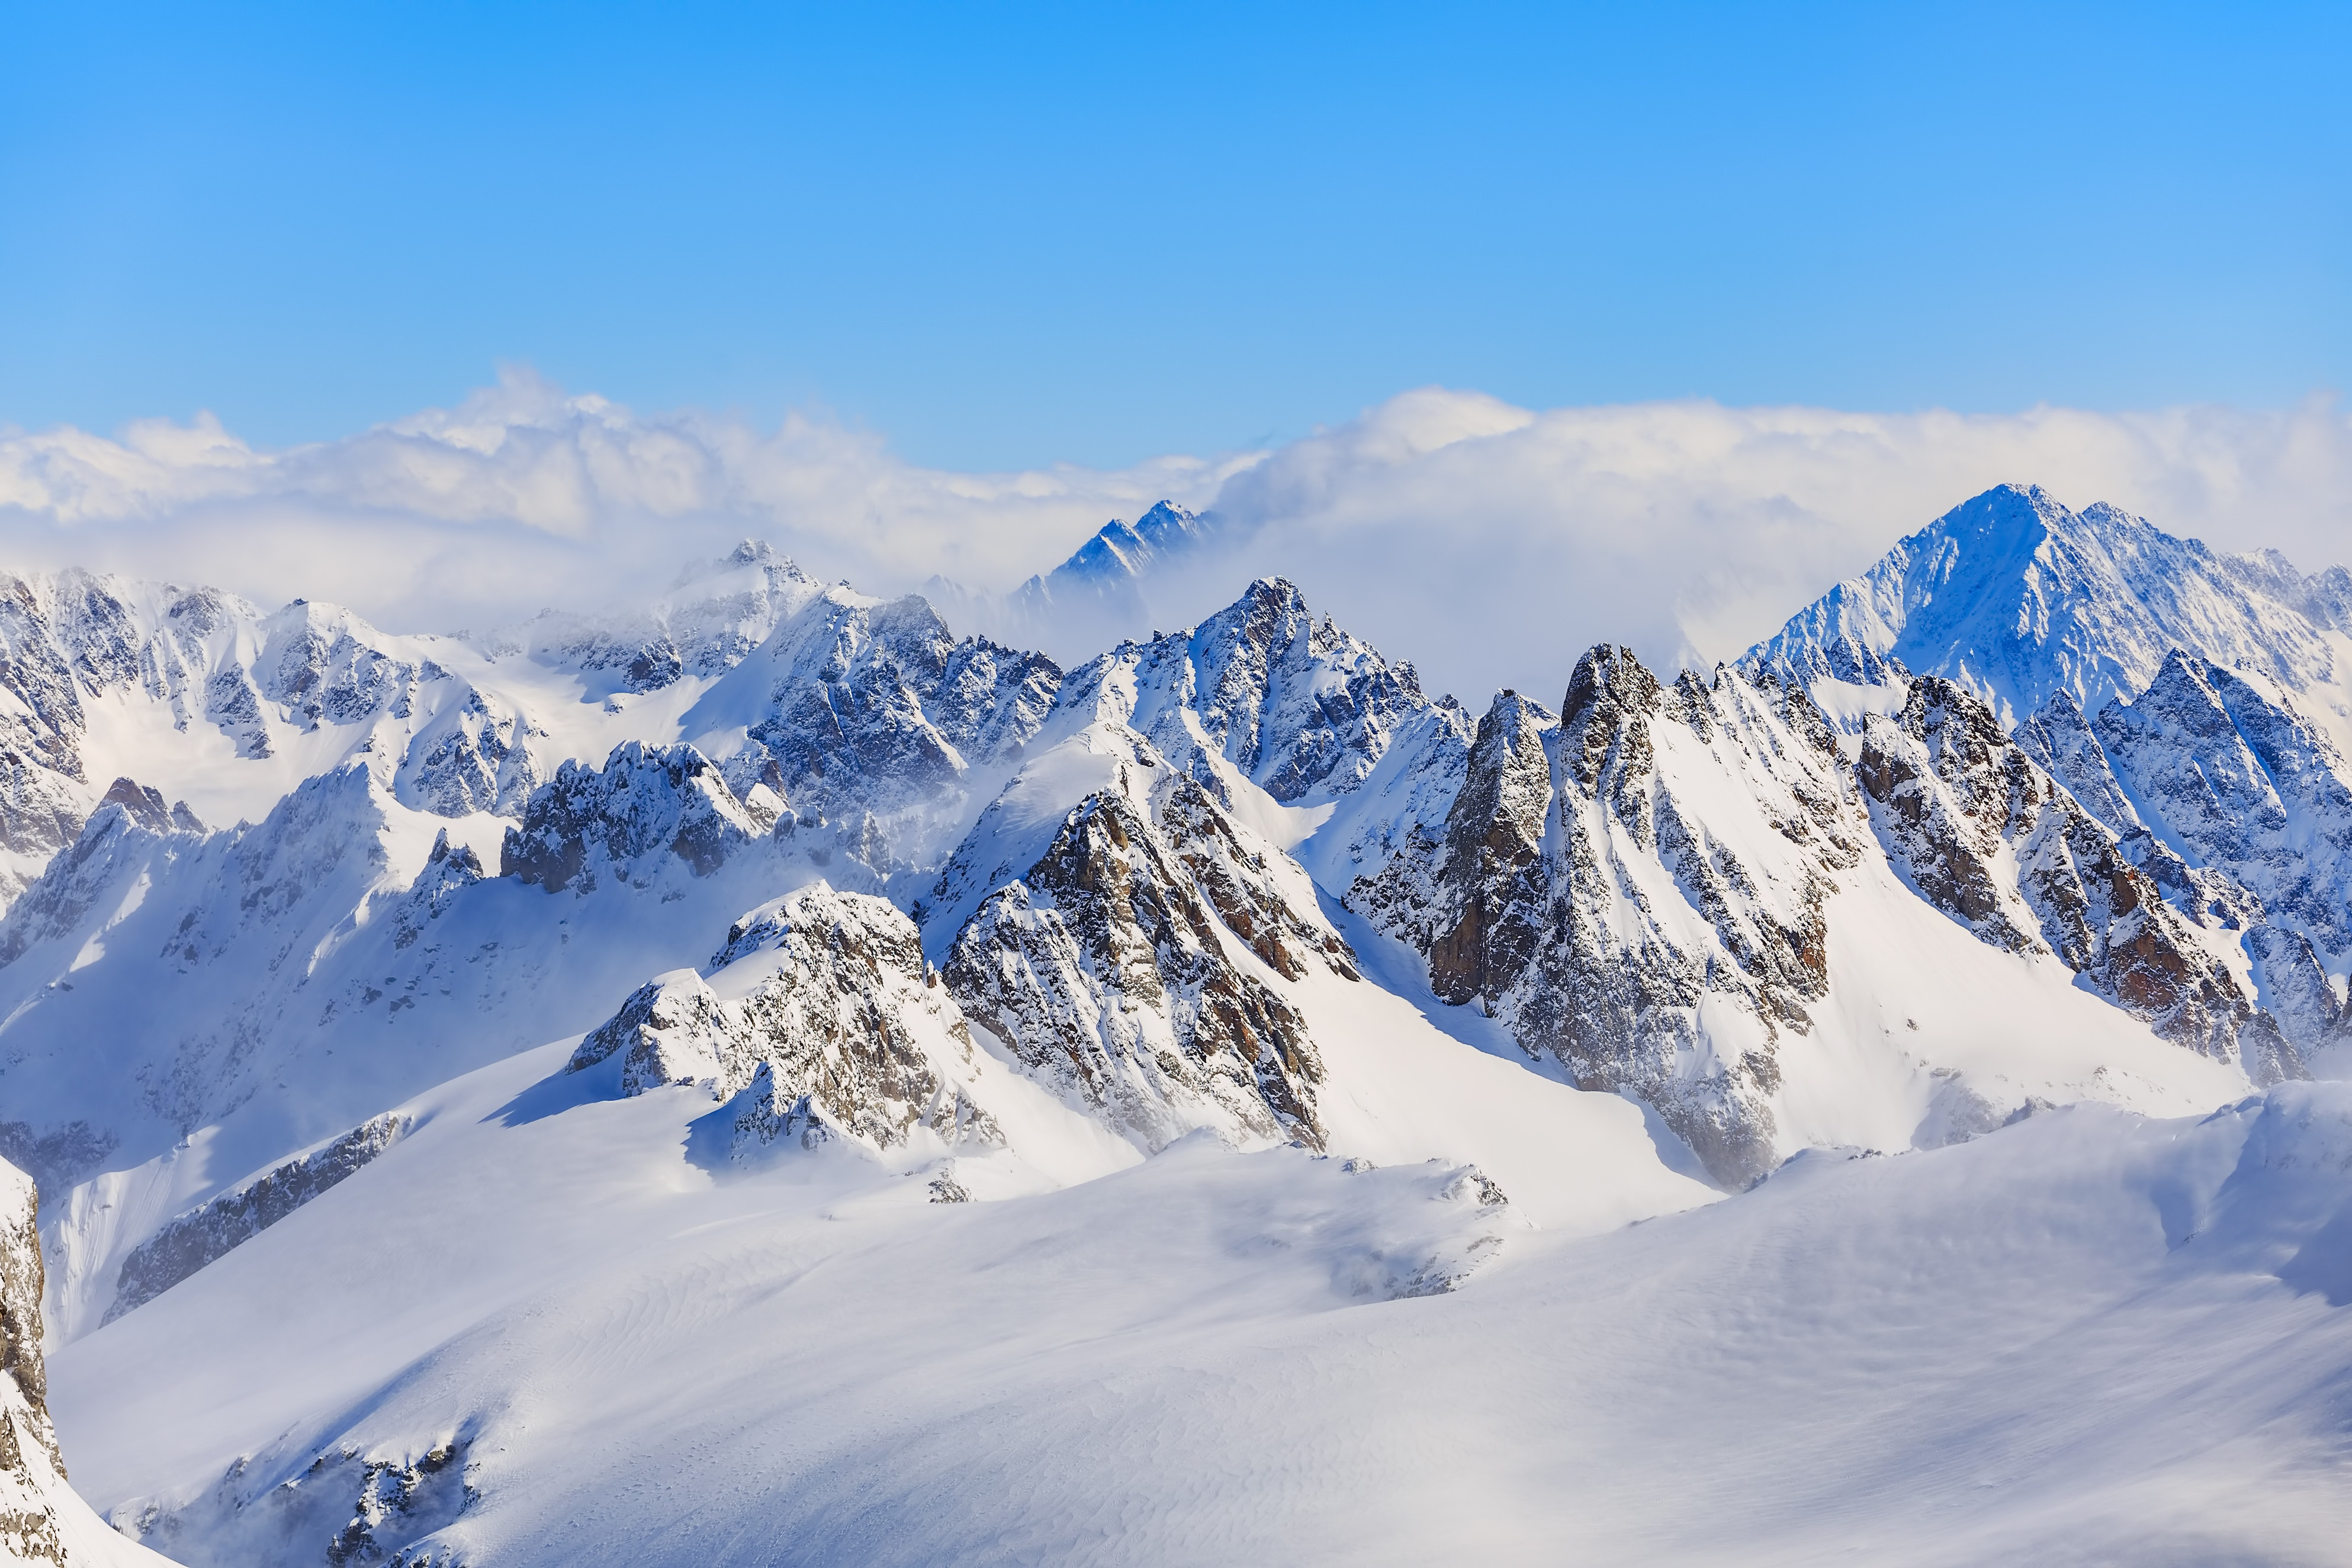
\includegraphics[scale=0.03]{mountain}
        \caption{\LaTeX 中的绘图}\label{fig-mountain}
    \end{figure}

    熟练使用\LaTeX 中的Tikz,可以绘制如图\ref{fig=tikz}所示的精美矢量图
    \begin{figure}[htbp]
        \centering
        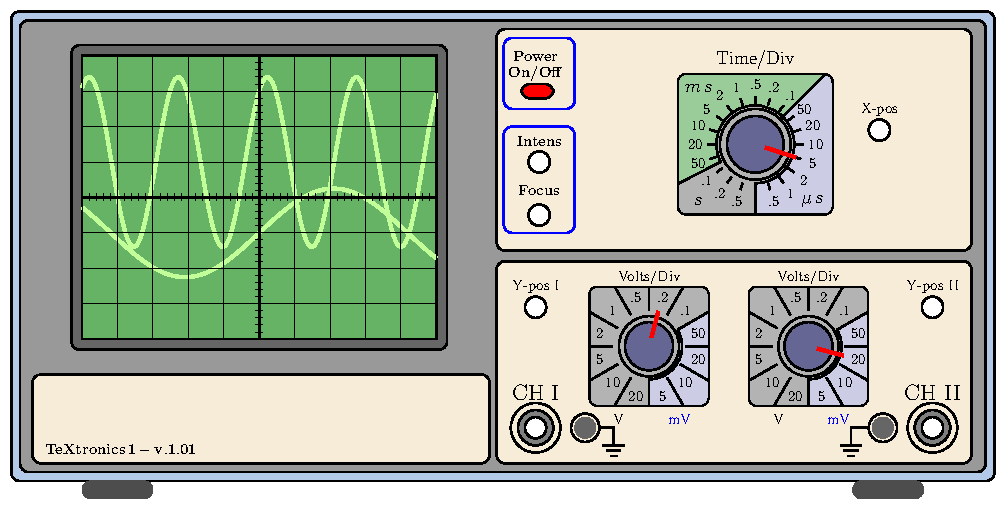
\includegraphics[scale=0.3]{oscilloscope}
        \caption{\LaTeX 中的绘图}\label{fig=tikz}
    \end{figure}

    当然,在\LaTeX {}中也可以使用表\ref{tab-score}所示的表格。
    \begin{table}[h]
        \centering
        \caption{考试成绩单}\label{tab-score}
        \begin{tabular}{|l|c|c|c|r|}
            \hline
            姓名 & 语文 & 数学 & 英语 & 备注 \\
            \hline
            张三 & 87 & 100 & 93 & 优秀 \\
            \hline
            李四 & 75 & 64 & 52 & 补考另行通知 \\
            \hline
            王五 & 80 & 82 & 78 & \\
            \hline
        \end{tabular}
    \end{table}

\end{document}